% !TEX encoding = UTF-8
% !TEX TS-program = pdflatex
% !TEX root = ../tesi.tex

%**************************************************************
\chapter{Development of the tools}
\label{cap:tools}
In this chapter, the study behind the development of every single created tool will be explained, and technical details about implementation.
%**************************************************************

\section{Tool for automated creation of attacker's profile}
This section reports the study and development process of the tool for the automated creation of an attacker profile.

\subsection{The tool: \texttt{create-profile.py}}
\label{cap:tool-create}
The attacker profiles were created from the various profile category configurations identified in Chapter \ref{cap:table-configuration}. The process is automated, that is, using a tool, called ``\texttt{create-profile.py}'', which after requesting specific values as input, responds in output with a complete card of the attacker profile's personal data.
\par \noindent The tool, run from the terminal, requires as input:
\begin{itemize}
	\item \texttt{cod\_id},\par \noindent an identification code to identify the profile in a simpler way (with this parameter, \texttt{PF-}\textit{n} will be created, where \textit{n} is this \texttt{cod\_id}).\par \noindent Accepted values: numeric parameter (\texttt{int});
	
	\item \texttt{gender},\par \noindent i.e., the gender of the attacker\par \noindent Accepted values: string parameter $s$, with $s \in \{$\texttt{female, male}$\}$;
	
	\item \texttt{real\_img},\par \noindent boolean value for the type of image profile the attacker must have.\par \noindent Accepted values: boolean parameter (\texttt{true} or \texttt{false});
	
	\item \texttt{age},\par \noindent i.e., the age of the attacker.\par \noindent Accepted values: numeric parameter (\texttt{int});
	
	\item \texttt{agehide},\par \noindent boolean value for whether the age will be visible in the profile or not.\par \noindent Accepted values: boolean parameter (\texttt{true} or \texttt{false}).
\end{itemize}
\par \noindent  Moreover, the tool use datasets (created ad hoc) to generate a most complete and realistic profile possible:
\begin{itemize}
	\item \texttt{dataset-name.json}, to randomly assign the name to the profile, based on the input \texttt{gender} parameter; this dataset is formed with the most common Italian names, both male and female, more than 100 for each.
	\item \texttt{dataset-surname.json}, to randomly assign the surname to the profile; this dataset is formed with the 100 most common Italian surnames.
	\item \texttt{dataset-city.json}, containing the list of Italian provinces to randomly assign the city of residence to the profile;
	\item \texttt{dataset-occupation.json}, to randomly assign the job occupation to the profile;
\end{itemize} 

\subsection{Development of the tools}
\begin{itemize}
	\item First of all, using \texttt{dataset-name.json}, a random name is extract and assign to the profile, based on the input \texttt{gender} parameter. Same thing for the surname where, using \texttt{dataset-surname.json}, a random surname is extract and assign to the profile.
	\item After that, \texttt{real\_img} parameter and \texttt{gender} parameter will be check, and, the label to identify the attacker the label begins to be created.
	\item With the \texttt{age} parameter, the tool will then create an appropriate date of birth to be entered in the Facebook profile, both in the case \texttt{agehide} parameter is ``\texttt{true}'' or ``\texttt{false}'', because to register on Facebook it is necessary to enter a date of valid birth. \par \noindent With the correct age range, the last character of the label could be set now, so the \textit{label} is created.
	\item Despite \texttt{residence} and \texttt{occupation} are superfluous parameters fot this case of study, to make each attacker profile more complete and realistic, actual values were nevertheless entered, which obviously were not valued in the analysis for research purposes. \par \noindent About \texttt{occupation}, a minimum of control has been included, to make it consistent with age and leaving aside some special cases: each profile under the age of 18 will have a ``\texttt{Studentessa}'' or ``\texttt{Studente}'', while each profile over the age of 65 will have ``\texttt{Pensionata}'' or ``\texttt{Pensionato}'' as occupation. \par \noindent About \texttt{residence}, an attempt was made to scatter the various attacker profiles throughout the Italian peninsula. This was done in order not to risk having more attacker profiles in too close areas.
	\item Afterwards, the tool uses the temporary \textit{fake email generator service}\parencite{site:fake-email} to create the fake email with which this profile will then log into Facebook. The username of the email is made up of \texttt{nome.cognome.age}, for each profile. The tool will go to the temporary false email generator site, enter the username created in the appropriate input section and then save the complete email with the random domain that the site will propose.
	\item Consequently, the tool generates a password of 6 characters, formed by an uppercase letter, 4 lowercase letters, 2 numbers, and a special character, to use to log into Facebook.
	\item In the end, the tool generate the identification \textit{code} with the \texttt{cod\_id} (for example \texttt{PF-3}), and save the data in the dataset \texttt{attacker\_profiles.json}.
\end{itemize}
 
\subsection{Create Facebook accounts}
Originally, one idea was to create the Facebook account in an automated way, using a tool developed ad hoc. Unfortunately, however, in the study phase, it was seen how the social network applies very strict policies that often constrained the creation of these profiles. First of all, it required to enter a code that he would send by email and occasionally forced the resolution of a ReCAPTCHA to continue. Sometimes the email with the code not arrived, so the procedure broke up and the profile was blocked. In other cases, Facebook continued to ask to resolve ReCAPTCHAs, even though they were always resolved correctly, and, after a while, the profile was blocked.
\par \noindent Therefore, the creation is done manually, but, despite this, there were still some significant problems: in fact, many profiles, after entering the initial data were immediately blocked and could only be unlocked by entering a mobile number. So it was necessary frequently changing browser, connection, device, operating system, and even site for the generation of temporary emails. To avoid running into further blocks, the profiles were created gradually, that is, days apart from each other.
\par \noindent Once created, each profile was included in numerous Facebook groups of different genres (reading, music, sports, etc.) and occasionally some content was shared in their personal profile.
\par \noindent Furthermore it's important to underline that some profiles with \texttt{real\_img} parameter set as \texttt{false} are minors, although in Chapter 5.1.3 it can be seen how the 3 age ranges only consider adult people. This was done because the age of these profiles, as evidenced by the corresponding \textit{label}, is not visible to the victim profiles who find the friend request, as the age is hidden.
\par \noindent The last step concerns the profile picture. It is necessary to specify that the profile pictures where the \texttt{real\_img} parameter is set to \texttt{true} are not of real people, as they were fished a site that generates realist pictures of a person\parencite{site:fake-img}. It generates a realistic picture of a person every time the page is refreshed, using artificial intelligence. So, the profile pictures were obviously chosen after creating every single attacker profile with the tool, because it was necessary to be consistent with the age of the profile user.
\par \noindent In the end, the profile pictures where the \texttt{real\_img} parameter is set to \texttt{false} were chosen looking random images in Google Images.
\par \noindent The 12 attacker profiles that have been generated are reported on Table \ref{table:attackers}.
\begin{table}[H]
	\centering
	\caption{Attacker profiles generated with the \texttt{create-profile.py} tool (see Chapter \ref{cap:tool-create}) and used for this project.}
\begin{tabular}[c]{ |c|c|m{1.5cm}|c|c|c|c|m{1.85cm}| } 
	\hline
	\cellcolor[HTML]{b0d7ff}\textsc{cod} & 
	\cellcolor[HTML]{b0d7ff}\textsc{label} & 
	\multicolumn{1}{|c|}{\cellcolor[HTML]{b0d7ff}\textsc{img}}&
	\cellcolor[HTML]{b0d7ff}\textsc{name} & 
	\cellcolor[HTML]{b0d7ff}\textsc{surname} &
	\cellcolor[HTML]{b0d7ff}\textsc{age} &
	\cellcolor[HTML]{b0d7ff}\textsc{residence}	&
	\cellcolor[HTML]{b0d7ff}\textsc{occupation}	\\
	%\cellcolor[HTML]{e6f2ff}
	\hline
	\cellcolor[HTML]{b0d7ff}\texttt{PF-0}&\cellcolor[HTML]{e6f2ff}\texttt{MT4}&	
	\vspace{.15cm}
	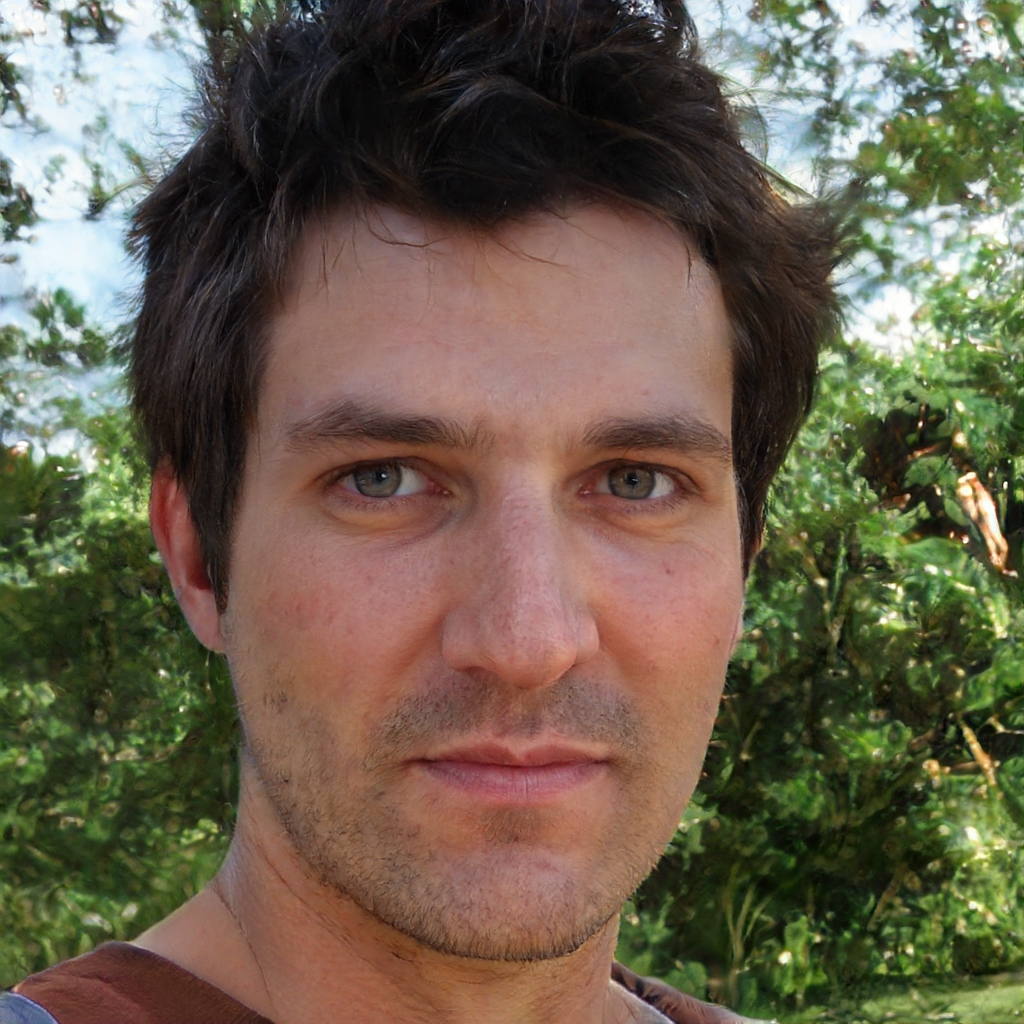
\includegraphics[height=1.5cm]{immagini/MT4.jpg}
	&Giuseppe&Martini&39&Ancona&Farmacista\\
	\hline
	\cellcolor[HTML]{b0d7ff}\texttt{PF-1}&\cellcolor[HTML]{e6f2ff}\texttt{MF4}&	
	\vspace{.15cm}
	
\includegraphics[height=1.5cm]{immagini/MF4.jpg}
	&Alessio&Fontana&17&Pescara&Studente\\	
	\hline 
	\cellcolor[HTML]{b0d7ff}\texttt{PF-2}&\cellcolor[HTML]{e6f2ff}\texttt{MF2}&	
	\vspace{.15cm}
	
\includegraphics[height=1.5cm]{immagini/MF2.jpg}
	&Samuel&Colombo&44&Caserta&Tappezziere\\
	\hline
	\cellcolor[HTML]{b0d7ff}\texttt{PF-3}&\cellcolor[HTML]{e6f2ff}\texttt{MT3}&	
	\vspace{.15cm}
	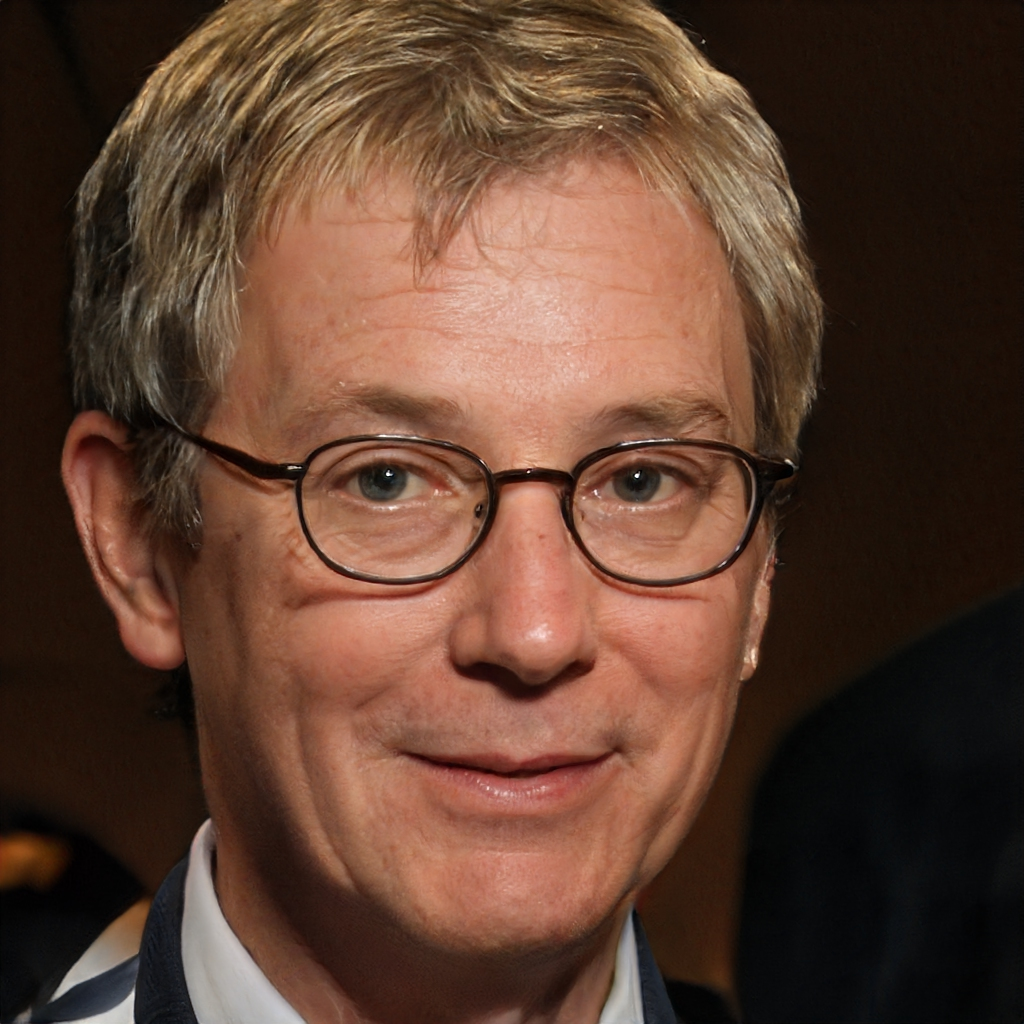
\includegraphics[height=1.5cm]{immagini/MT3.jpg}
	&Carlo&De Angelis&57&Siena&Chimico\\	 	
	\hline
	\cellcolor[HTML]{b0d7ff}\texttt{PF-4}&\cellcolor[HTML]{e6f2ff}\texttt{MF3}&	
	\vspace{.15cm}
	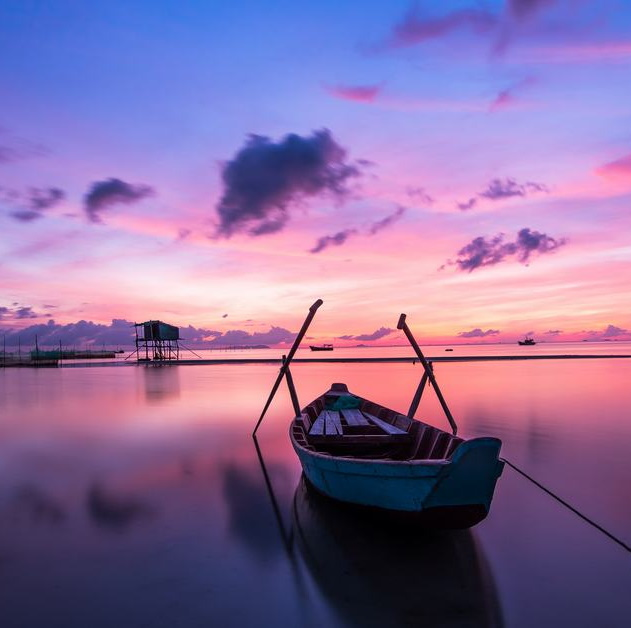
\includegraphics[height=1.5cm]{immagini/MF3.jpg}
	&Valerio&Mazza&57&Catanzaro&Dentista\\
	\hline 		
	\cellcolor[HTML]{b0d7ff}\texttt{PF-5}&\cellcolor[HTML]{e6f2ff}\texttt{MT2}&	
	\vspace{.15cm}
	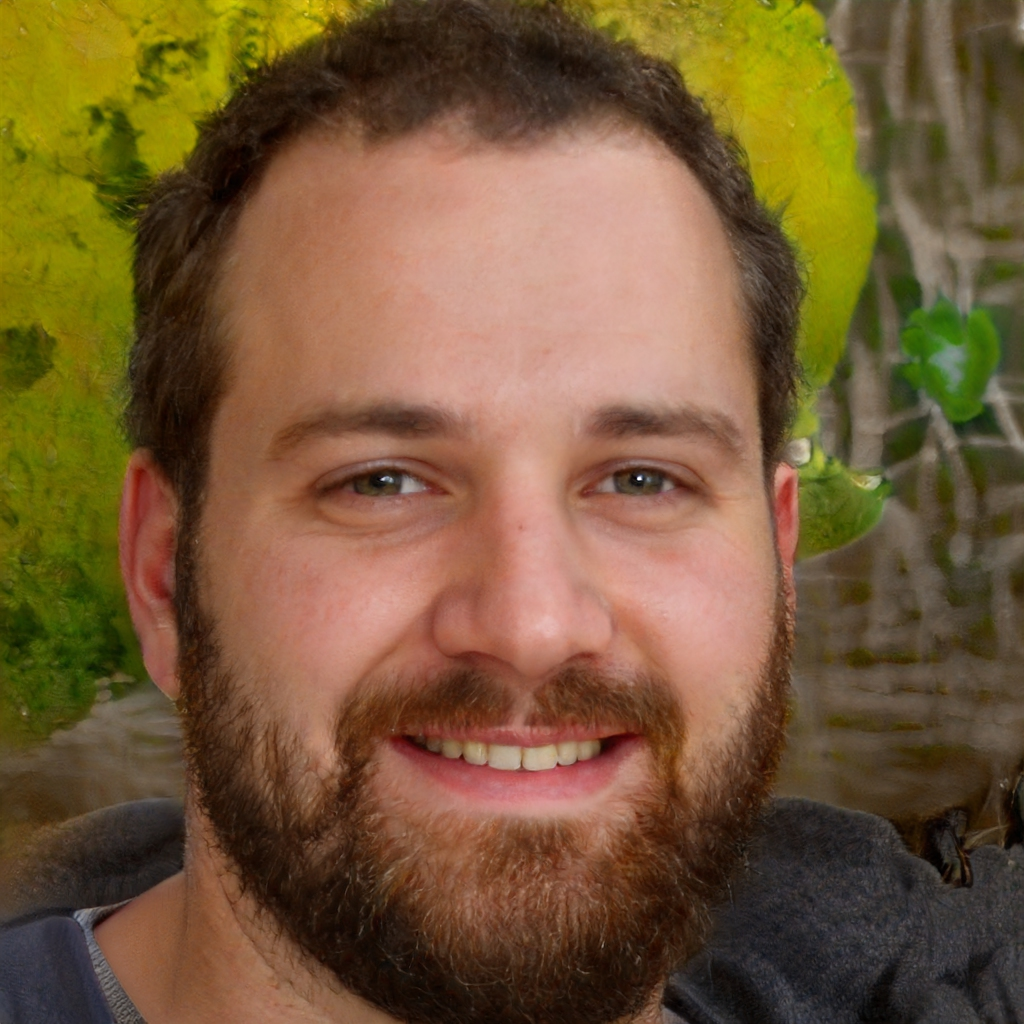
\includegraphics[height=1.5cm]{immagini/MT2.jpg}
	&Leonardo&Neri&45&Roma&Tatuatore\\
	\hline
	\cellcolor[HTML]{b0d7ff}\texttt{PF-6}&\cellcolor[HTML]{e6f2ff}\texttt{FT4}&	
	\vspace{.15cm}
	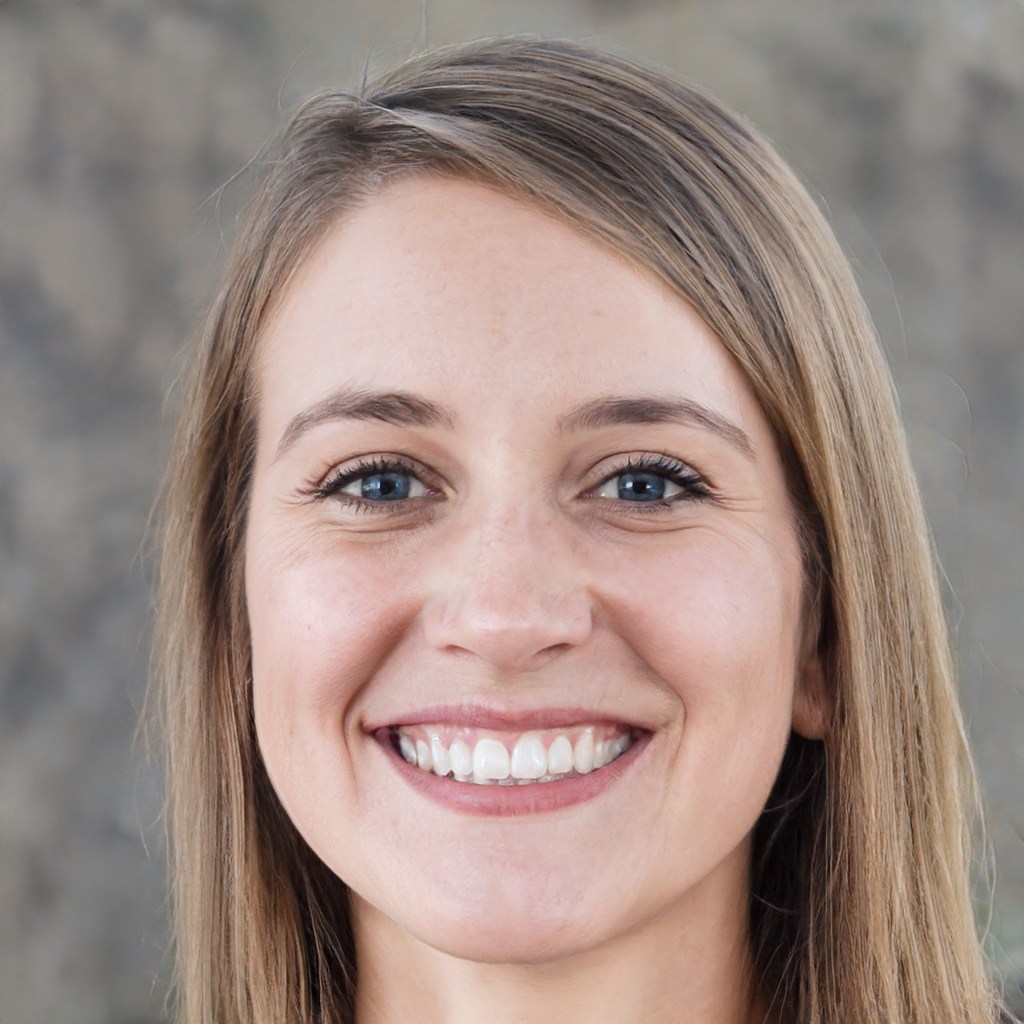
\includegraphics[height=1.5cm]{immagini/FT4.jpg}
	&Giulia&Ferrari&32&Palermo&Istruttrice di Yoga\\ 
	\hline
	\cellcolor[HTML]{b0d7ff}\texttt{PF-7}&\cellcolor[HTML]{e6f2ff}\texttt{FF4}&	
	\vspace{.15cm}
	
\includegraphics[height=1.5cm]{immagini/FF4.png}
	&Michela&D'Angelo&16&Taranto&Studentessa\\
	\hline
	\cellcolor[HTML]{b0d7ff}\texttt{PF-8}&\cellcolor[HTML]{e6f2ff}\texttt{FF2}&	
	\vspace{.15cm}
	
\includegraphics[height=1.5cm]{immagini/FF2.png}
	&Ilaria&Riva&26&Verona&Stilista\\	
	
	\hline
	\cellcolor[HTML]{b0d7ff}\texttt{PF-9}&\cellcolor[HTML]{e6f2ff}\texttt{FT3}&	
	\vspace{.15cm}		
	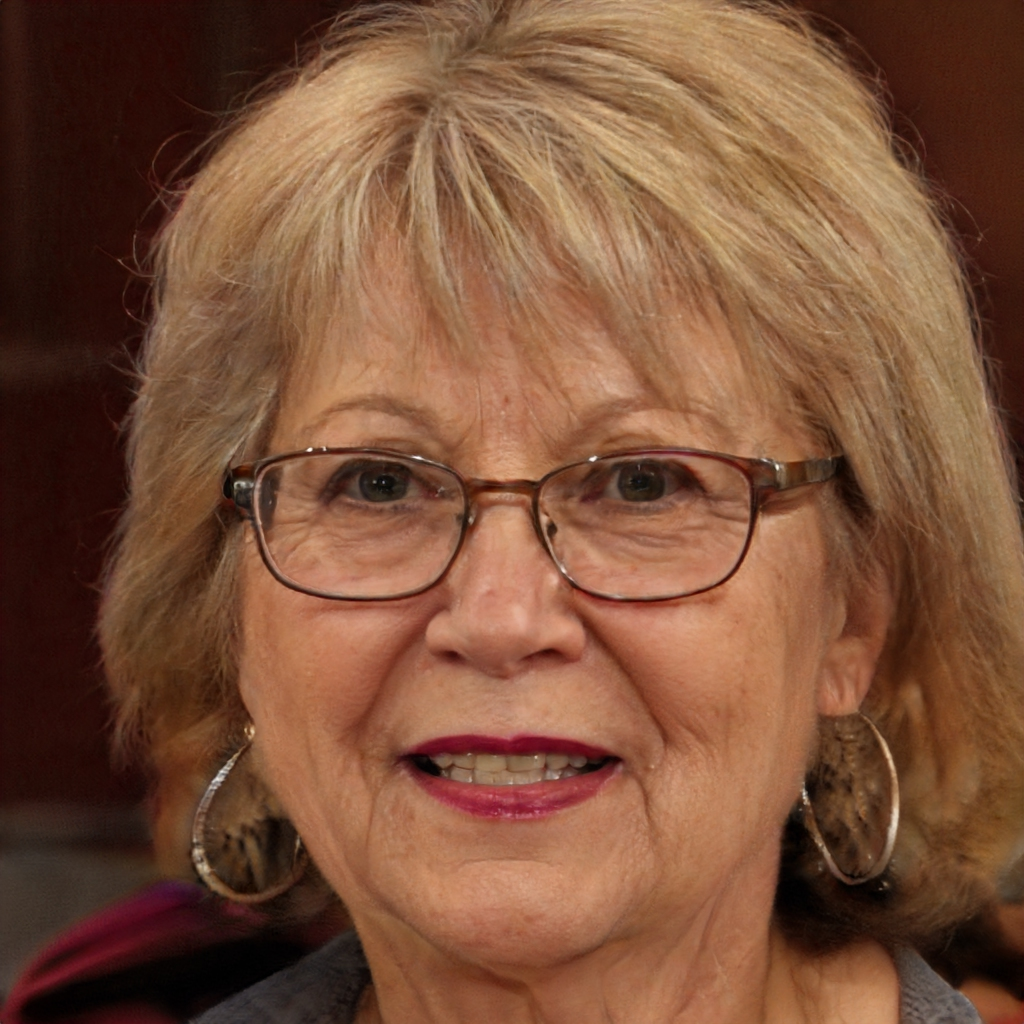
\includegraphics[height=1.5cm]{immagini/FT3.jpg}
	&Giulia&Moro&72&Vercelli&Pensionata\\
	
	\hline
	\cellcolor[HTML]{b0d7ff}\texttt{PF-10}&\cellcolor[HTML]{e6f2ff}\texttt{FF3}	&
	\vspace{.15cm}
	
\includegraphics[height=1.5cm]{immagini/FF3.jpg}
	&Sara&Rizzo&59&Bologna&Fiorista\\
	\hline
	\cellcolor[HTML]{b0d7ff}\texttt{PF-11}&\cellcolor[HTML]{e6f2ff}\texttt{FT2}	&
	\vspace{.15cm}
	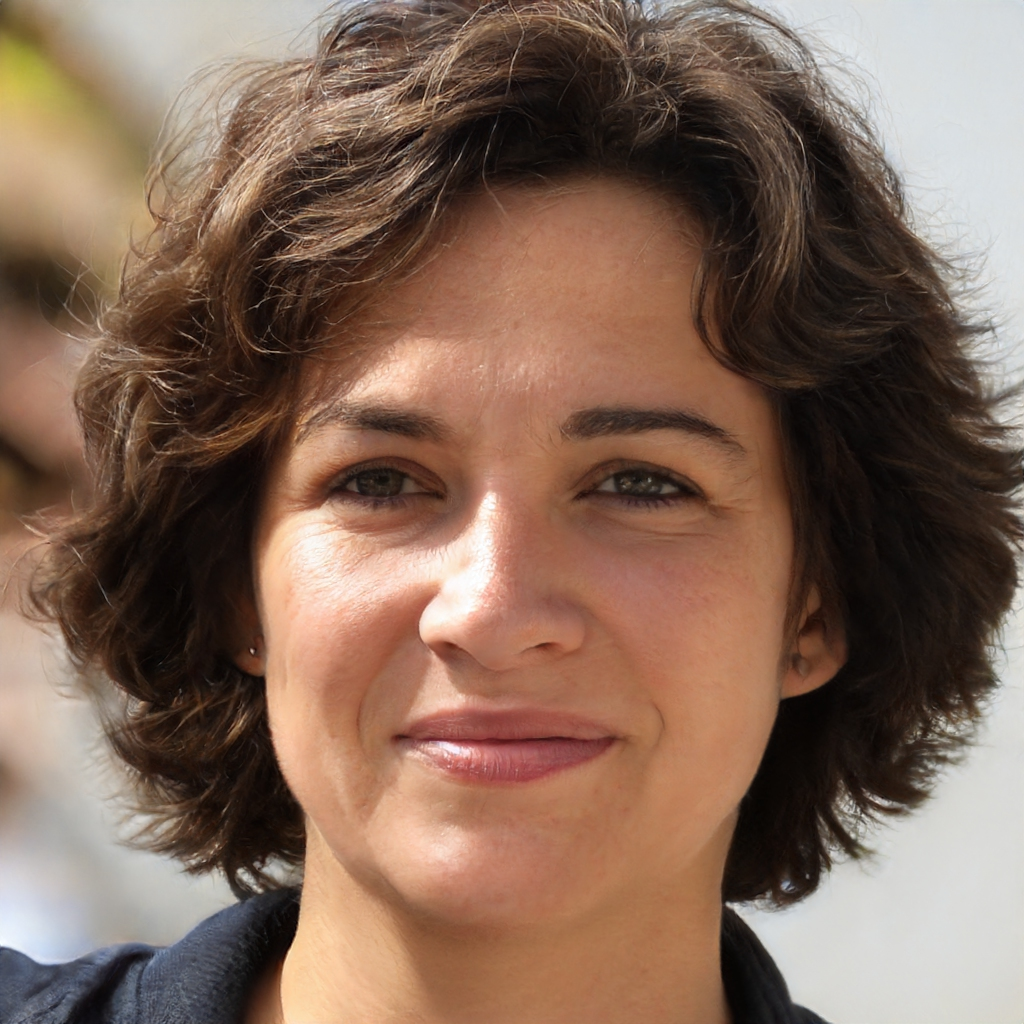
\includegraphics[height=1.5cm]{immagini/FT2.jpg}			
	&Federica&Grasso&38&Milano&Agente \newline Assicurativo\\	
	 \hline	 	
\end{tabular}
\label{table:attackers}	 
\end{table}
\newpage
\section{Tool for automated search of a victim's profile}
This section reports the study and development process of the tool for searching for a victim profile in an automated way.\par \noindent 
The initial idea was to develop a tool that would scrape and categorize the profiles at the same time they are searched for. For example, the tool logs into Facebook with the credentials of an attacker profile, somehow it gets a list of possible victim profiles and, one by one, it enters on it to scrape and categorize it, saving the result in the appropriate file. This means that the tool would move to the next profile until the list is over. Computationally, this process is long and cumbersome, scraping would have increased significantly and, above all, this procedure is all done with a single attacker profile: this could be bring Facebook to block it, as it would always perform the same action in a loop for a long time.
\par \noindent Furthermore, the Facebook search interface is not helpful for this case study, as it gives the possibility to set the parameters of ``city'', ``education'', ``work'' and ``friends of friends'', and these parameters have nothing to do with this case study. \par \noindent 
For all these reasons, it was necessary to proceed differently: first using a tool called \texttt{get-list-profile.py} to save a list of eligible victim profiles and then a subsequent tool called \texttt{classificator-profile.py} which determines for each profile if and what kind of victim it is.
\par \noindent The idea and operation of these two tools are now explained in detail.

\subsection{The tool: \texttt{get-list-profile.py}}
This first tool saves a list of profiles which will then be analyzed and classified by the next tool.\par \noindent In detail, the tool, run from the terminal, requires as input:
\begin{itemize}
	\item \texttt{cod\_id}, that's the attacker's profile code;
	\item \texttt{type\_victim}, i.e., gender of the victim profiles that will be collect.\par \noindent Accepted values: string char $s$, with $s \in \{$\texttt{f, m}$\}$;.
\end{itemize}
First of all, the tool examine the attacker's \texttt{cod\_id} to verify that it exists and, if so, save its email and password to log in to Facebook. This is because it is not possible to search for profiles on Facebook without logging in.
\par \noindent At this point, based on the gender entered in the input, the tool randomly chooses a name from \texttt{dataset-names.json} and searches that name. Facebook responds by showing a list of profiles with that name. But, more precisely, Facebook would show a list of profiles residing in a circumstantial area to that of the profile with which you are searching. To broaden the search range, we have chosen to use provinces instead of cities (and therefore to insert only the Italian provinces within the \texttt{dataset-city.json} dataset) and to disperse the attacker profiles throughout the Italian territory. 
\par \noindent Furthermore, each attacker profile searched for a minimum of 4 different named profiles with \texttt{gender = ``f''} (i.e., \textit{female}) and a minimum of 4 different named profiles with \texttt{gender = ``m''} (i.e., \textit{male}). A minimum or maximum limit was not given to the profiles to be collected, also because they were not yet assigned to the corresponding label.
\par \noindent In any case, from the list of resulting profiles, the tool clicks on the ``Show all'' button to load an even greater number of profiles and, scrolling the page a couple of times, saves in a \texttt{file} all user-profiles' url with the searched name.
\par \noindent Several copies of this tool have been created, which differ from each other for the file where they save the list of profiles. This was done to be able to work in parallel, in order to collect as many profiles as possible in the shortest possible time.

\subsection{The tool: \texttt{classificator-profile.py}}
\label{cap:classificator-profiles}
This second tool analyzes each profile of a given list (output of the previous tool) to be able to attach to each of them its corresponding label, and then save them in the appropriate dataset, called \texttt{victims.json}.\par \noindent In detail, the tool, run from the terminal, requires as input:
\begin{itemize}
	\item \texttt{cod\_id}, that's the attacker's profile code;
	\item \texttt{file}, that's the name of the file containing the list of victim profiles that must be analyzed and categorized.
\end{itemize}
First of all, the tool examine the attacker's \texttt{cod\_id} to verify that it exists and, if so, save its email and password to log in to Facebook. This is because it is not possible to search for profiles on Facebook without logging in.
\par \noindent At this point, the tool opens the correct file based on the \texttt{file} parameter passed in input (the file is in the same folder as the tool).
It reads line by line, taking each URL that will lead to a saved victim profile.\par \noindent Once the URL has been selected, the tool moves to the dashboard of this profile, in order to analyze its details. Here, the tool first checks for the presence of the button to add the profile to friends: some profiles do not allow you to be added to friends, but you can only follow them or send a private message. If the button is present, it will continue the analysis, otherwise, it will go to the next URL.
\par \noindent  As a first point, the tool checks the profile picture.
The algorithm uses the \texttt{alt} of the profile image to identify the presence (or not) of people within the image, a sufficient condition to make the \texttt{real\_img} parameter as \texttt{true} (details in Chapter \ref{cap:alt-technology}). So, once it have checked the \texttt{alt} of the profile image, the tool will declare the value of \texttt{real\_img} parameter: il will set to ``\texttt{T}'' in the case of the profile image contains at least one person, otherwise it will set to ``\texttt{F}''.
\par \noindent After that, the tool will have to analyze what kind of URL the victim profile has. In fact, there are two types of profile URLs:
\begin{itemize}
	\item \texttt{https://www.facebook.com/profile.php?id=\textit{numerical\_sequence}}\par \noindent \textit{e.g. https://www.facebook.com/profile.php?id=3322661122}
	
	\item \texttt{https://www.facebook.com/\textit{character\_string}}\par \noindent (sometimes followed by \texttt{.\textit{numerical\_sequence}})\par \noindent \textit{e.g. https://www.facebook.com/mario.rossi.32}
\end{itemize}
Due to this difference, a check has been implemented to understand what type of URL you are dealing with and, consequently, the correct link is assigned to move within the profile to find the information.
\par \noindent At this point, the tool knows what type of URL it has to create for moving to the ``about'' page, where there is the basic information of the profile. 
\par \noindent Once here, thanks to a regular expression, the tool checks for the presence of a 4-character string, indicating the year of birth. If it is present, the age is calculated and the corresponding range between ``2'' or ``3'' is assigned, otherwise, the assigned range is ``4'' (details in Chapter \ref{cap:age-parameter}).
\par \noindent As a last step, the tool analyzes the gender of the profile, first looking for the presence of the string ``Female'' or ``Male'' and, if it is not found, it moves to \texttt{dataset-name.json} to search in which category that name is found. It will assign \texttt{F} if the profile is of a woman, \texttt{M} if it belongs to a man.
\par \noindent 
Once at this point, the tool has created the corresponding label and this is where the \textit{check system} comes into play: before categorizing the profile, it asks for manually checked via the terminal, showing the label created. If it is correct, it's necessary to answer affirmative (with an ``ok''), otherwise, the correct label must be enter.
\par \noindent Now, the tool has the exact label, so it can save the profile within the \texttt{victims.json} dataset, obviously after checking if that profile does not already exist.
\par \noindent Once the process is finished, move on to the next URL, until the list is over. Then, it destroys the \texttt{file} with the profile list and ends its execution.
\par \noindent A maximum limit for the profiles to have for each category has not been decided. On the contrary, a minimum number has been defined: each attacker profile will have to perform 3 friend requests for each category of victim profile (including the category in which it belongs). 
\par \noindent Considering that there are $12$ categories of attacker profiles, the minimum number of victim profiles for each category is $12 \cdot 3 = 36$ (so collect $12 \cdot 36 = 432$ victim profiles). An analysis tool aided this collection process, showing how many profiles were needed to reach the minimum value based on those already collected (details about the tool in Chapter \ref{cap:victims-analysis}). 

\newpage
\section{Tool for automated friend request}
\label{cap:tool-friend-request}
This section reports the study and development process of the tool for the automated friend request from an attacker profile to one or more victim profiles. This tool is the simplest in terms of implementation, as it was only necessary for it to log in and ask for friendship from a profile given in input. \par \noindent  
First of all, a series of considerations need to be made:
\begin{enumerate}
	\item each \textit{attacker} profile must send the friend request to 3 \textit{victim} profiles for each category;
	\item a \textit{victim} profile must not receive the friend request from more than one \textit{attacker} profile;
	\item each \textit{attacker} profile must have the same number of total friend requests to make;
	\item an \textit{attacker} profile mustn't send too many friend requests in close moments, because Facebook would block the profile.
\end{enumerate}
For this reason, first a tool called \texttt{round-add.py} was created and then the definitive friend request tool, called \texttt{add-friend.py}. 

\subsection{The tool: \texttt{round-add.py}}
This first tool must set the friendship requests that each \textit{attacker} profile has to send: it assigns to each attacker profile $36$ victim profiles to which to send the friend request. 
Each URL within the \texttt{victims.json} dataset is seen as an element of an array, and the name of the array is given by its category name.
\par \noindent  This tool must know:
\begin{itemize}
	\item the exact number of \textit{victim} profiles to witch each \textit{attacker} profile must send the friend request (36 in this case of study);
	\item the label of each \textit{victim} to witch one \textit{attacker} profile must send the friend request;
	\item the exact number of \textit{attacker} profile (12 in this case of study);
	\item the \texttt{cod} of each \textit{attacker} profile;
	\item the number of friend requests that each profile will have to send for each category (3 in this case of study).
\end{itemize}
The tool process this information and within the \texttt{set\_request.json} dataset, it will assign to each attacker profile the list of URLs of victim profiles to be attacked. It is nothing more than a list of positions of elements within each array containing the URL list of victim profiles. To calculate the index of each element, the numerical value of the \textit{attacker} profile is considered, to simulate a ``jump'' to the correct element, as many as there are attacker profiles available.\par \noindent 
At this point, each attacker profile has its personal list of victim profiles to attack and the next tool comes into play.
\par \noindent The tool, run from the terminal, does not need any input parameters.

\subsection{The tool: \texttt{add-friend.py}}
Given an attacker profile and its respective list of victim profiles that he will have to attack, this second tool takes care of requesting the friendship from the \textit{attacker} profile to the \textit{victim} profile.\par \noindent 
However to avoid being blocked by Facebook, it was decided to structure this attack in rounds: at each round, identified with an index, an attacker profile will have to send the friend request from \texttt{n} victim profiles.\par \noindent 
The tool point to the first element of the victim profiles list of one specific attacker profile, skipping the elements that are part of the previous rounds.
\par \noindent There is a list that specifies how many friend request must be sent in every round (values ranging from 1 friend request to 4 friend requests). The index of each elements of this list is the identification value of the round.\par \noindent 
For example, at the 3rd round, knowing the number of profiles to which must request friendship in the previous rounds, the sum of them point to the first element of the victim profiles list to which the current attacker profile must send the friend request in this round.
\par \noindent In detail, the tool, run from the terminal, requires as input:
\begin{itemize}
	\item \texttt{cod\_id}, that's the attacker's profile code;
	\item \texttt{round}, the numerical value that indicates the attack round to be satisfied.
\end{itemize}
At this point, each \textit{attacker} profile will log into Facebook and send the friend requests to the victim profiles taken from the correct portion of the list in that particular round. \par \noindent 
To manage this delicate phase more accurately, an excel file has been built to keep track of the rounds already executed.
\par \noindent Once the friend request has been sent to a \textit{victim} profile, before moving on to the next one, the tool saves the information in a dataset called \texttt{request\_log.json}: for each attacker profile, the list of attacked victim profiles are indicated, with its specific category.